% !TEX encoding = UTF-8 Unicode
% !TEX root = thesis-ex.tex

This section will discuss the dijet balance as measured by the ATLAS detector for \pbpb\ collisions at $\sqrtsnn = 2.76$ TeV \cite{Aaboud:2017eww}.
The dijet imbalance can be expressed in terms of $x_J$ defined as:

\begin{align}
x_J =  \frac{\pt_2}{\pt_1}
\end{align}
where $\pt_2$ and $\pt_1$ are the transverse momenta of the two highest-\pt\ jets in the event respectively.
The minimum $\pt_2$ considered is 25 GeV and the pair of jets are separated by $|\Delta\phi| > 7\pi/8$.
The dijet yields normalized by the number of jets and determined as $1/N_\mathrm{jets} dN/dx_J$ are presented as a function of $x_J$ for different centrality intervals, as well as different ranges for $\pt_1$.
%The measured distributions are further unfolded to remove detector resolution effects and allow comparison to theoretical models.

Figure~\ref{fig:xJ} shows the $x_J$ distribution for dijet pairs in \pp\ and \pbpb\ collisions in two different centrality bins and two $\pt_1$ ranges.
It can be seen that the dijet yields in \pp\ are peaked at unity and become narrower for larger $\pt_1$ ranges.
This reflects the fact that the effects of jet quenching are minimal and the higher-\pt\ jets are better balanced.
The dijet yields in peripheral \pbpb\ collisions are similar to the distributions from the \pp\ data, showing that the effects of quenching are smaller.
On the other hand, dijet yields in central \pbpb\ collisions are significantly broadened, reflecting the maximal  of jet quenching.
This is consistent with the picture of the individual jets in the dijet pair traversing different lengths in the QGP and hence losing different amounts of energy.
In fact, the distribution for \pbpb\ data is peaked at $x_J = 0.5$, implying that the jets are highly unbalanced.
It is further seen that higher \pt\ jets have a narrower $x_J$ distribution.
This suggests that the fractional energy loss decreases with increasing jet \pt. 
Similar jet asymmetry has been observed at both RHIC and the LHC \cite{PhysRevLett.119.062301, Aad:2010bu, Chatrchyan:2012gt, Chatrchyan:2011sx}.

\begin{figure}[htbp]
\begin{center}
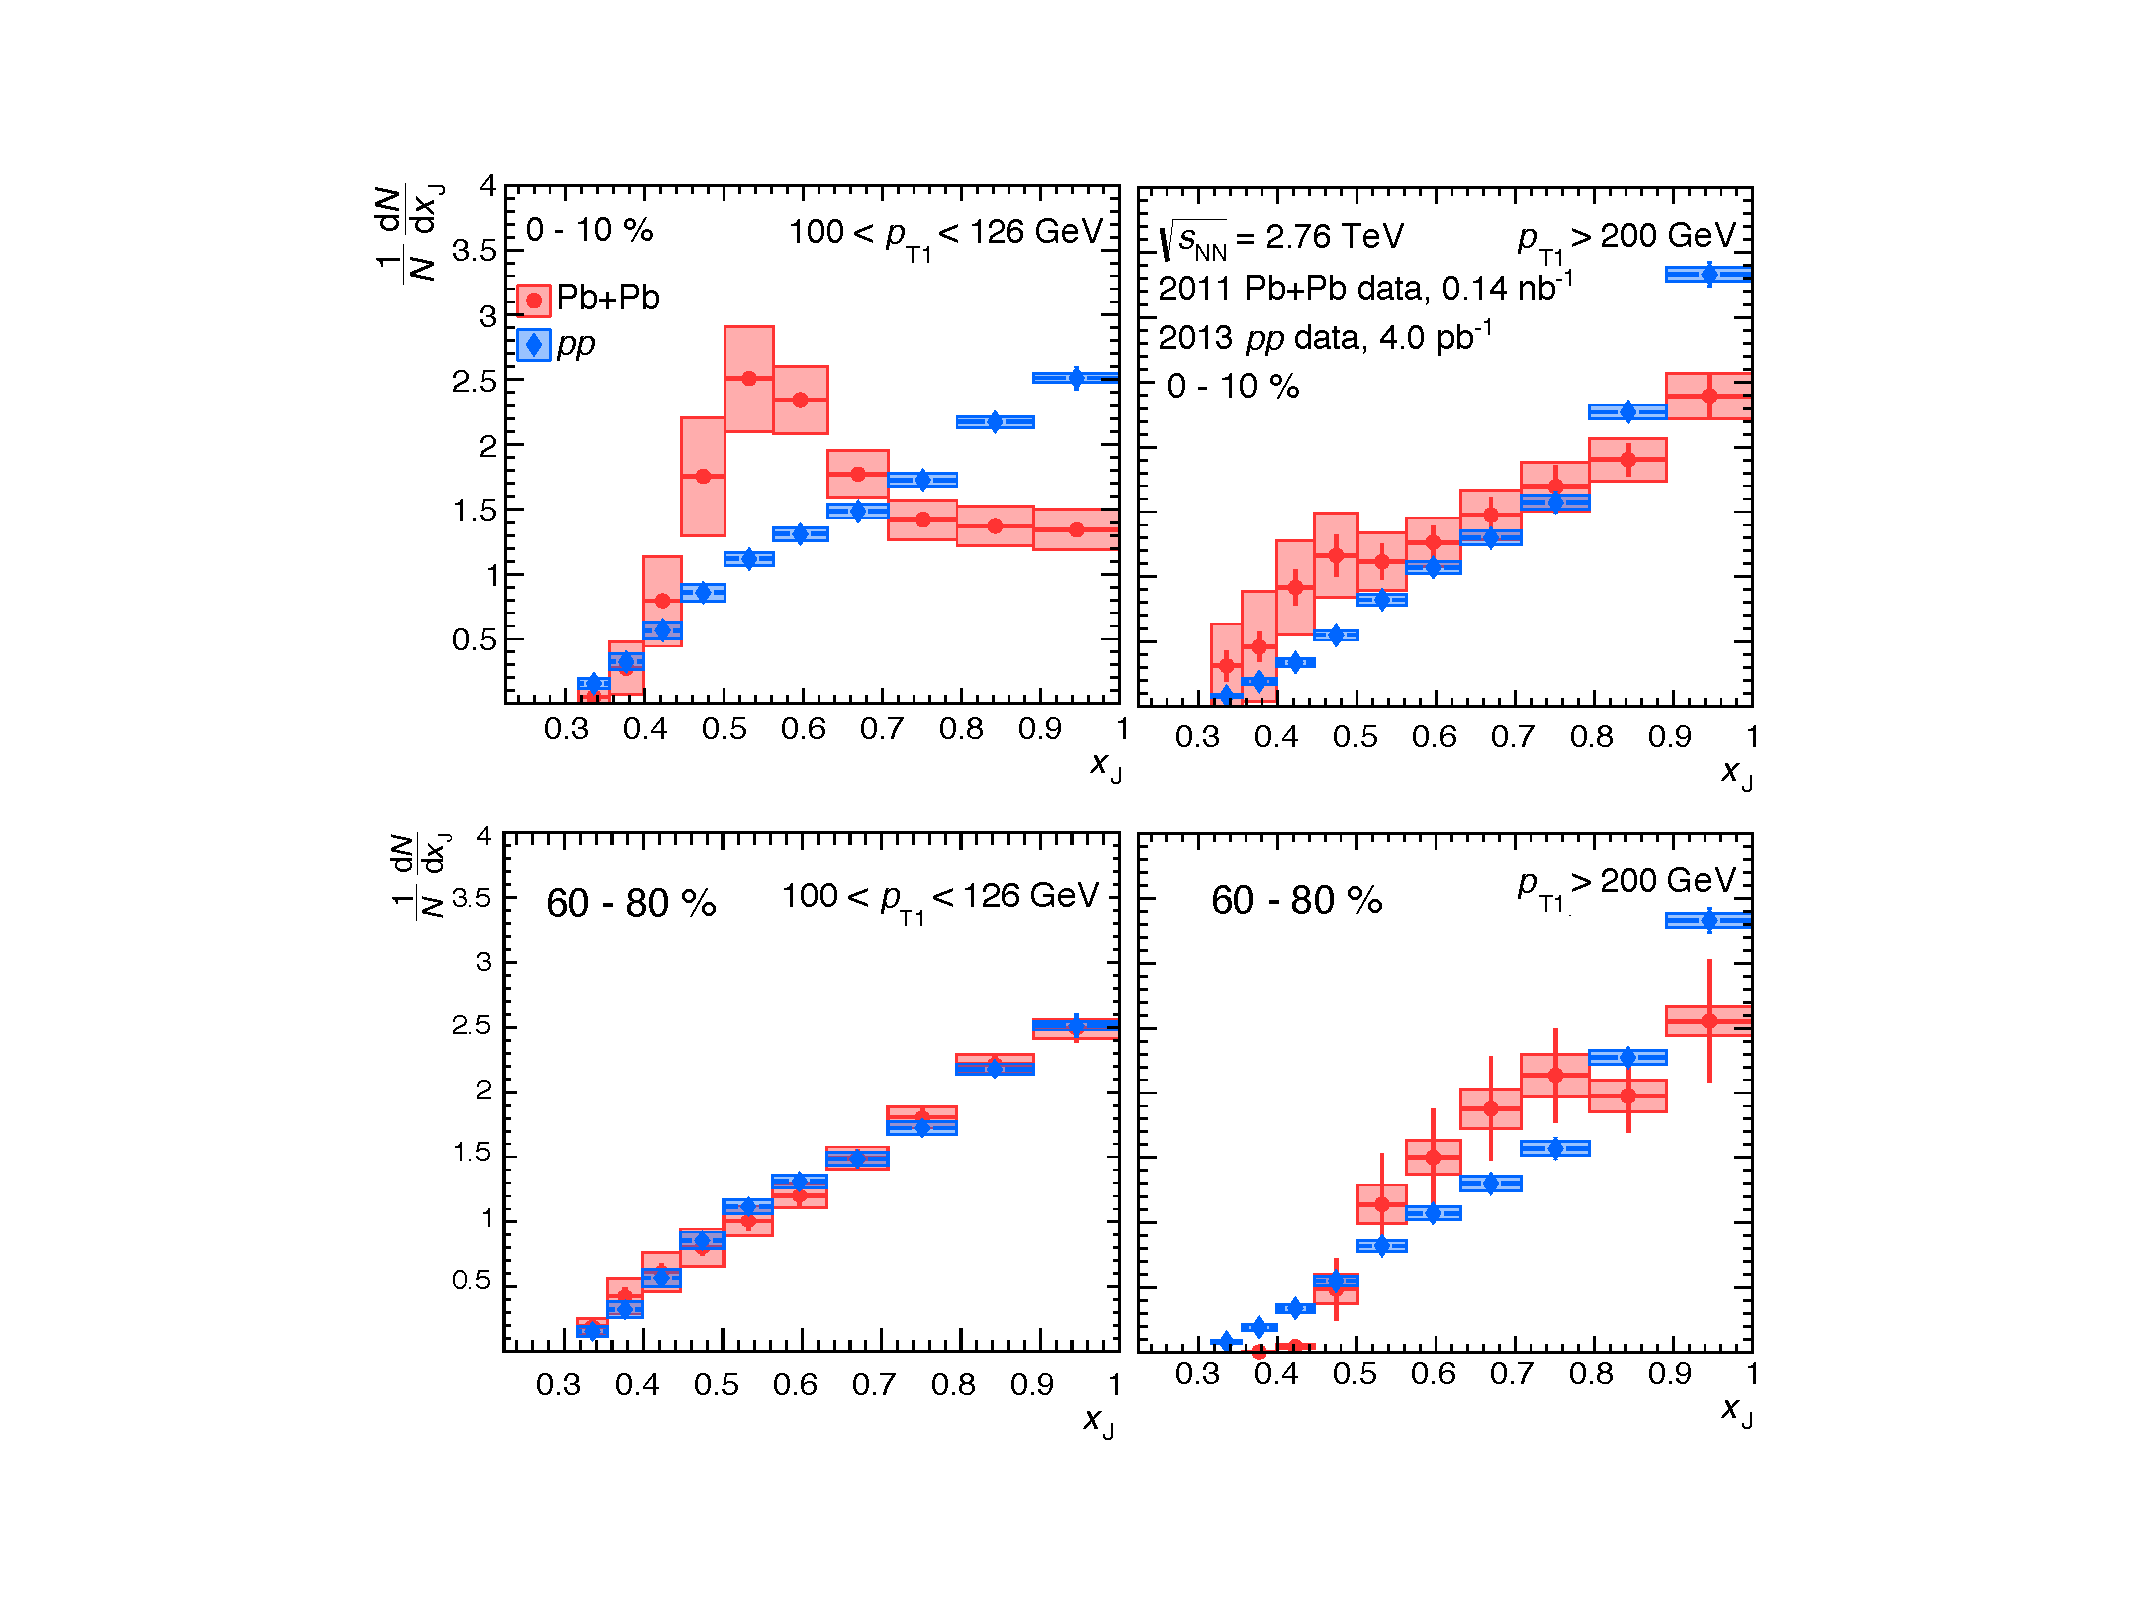
\includegraphics[width=0.55\textwidth]{figures/jetMeasurements/xJ}
\caption{The $1/N_\mathrm{jets} dN/dx_J$ distributions for $R=0.4$ jets as a function of $x_J$ for \pp\ (blue) and \pbpb\ (red) collisions.
The different panels are for (top) central and (bottom) peripheral collisions in (left) $100 < \pt_1 < 126$ GeV and (right) $\pt_1 > 200 $ GeV.
The \pp\ data is the same in all panels.
The statistical uncertainties are indicated by the bars while the boxes indicate the systematic uncertainties.
Figures from Ref.~\cite{Aaboud:2017eww}.}
\label{fig:xJ}
\end{center}
\end{figure}







%These distributions are significantly flatter than the ones for $R=0.4$ jets, an observation that is consistent with the expectation that the transverse momenta correlation between the dijet pair is weaker for jets with smaller radii due to radiation that is outside the nominal jet cone.

%\begin{figure}[htbp]
%\begin{center}
%\includegraphics[width=0.55\textwidth]{figures/jetMeasurements/xJ_R03}
%\caption{The $1/N_\mathrm{jets} dN/dx_J$ distributions for $R=0.3$ jets as a function of $x_J$ in \pp\ and central \pbpb\ collisions.
%The different panels are for different, $\pt_1$ ranges (top left to bottom right) central and (bottom) peripheral collisions.
%The \pbpb\ data is in red circles while the \pp\ data is in blue diamonds and is the same in all panels.
%The statistical uncertainties are indicated by the bars while the boxes indicate the systematic uncertainties.
%Figures taken from Ref.~\cite{Aaboud:2017eww}.}
%\label{fig:xJ_R03}
%\end{center}
%\end{figure}
%
